\section{Preliminaries}
\label{sec:preli}
% motivation
In the opportunistic network scenario,
the source node of the message always needs to 
disseminate the message, e.g., advertisement, urgent notification,
to the persons as many as possible.
As an example, the source node $src$ 
needs to disseminate its message $m$
to vehicles or pedestrians.
The $N$ relay nodes can replicate $m$
and send it to the vehicles,
which is shown in Fig.~\ref{fig:sketch}.
Thus the potential coverage area of the message
can be broadened by the opportunistic network.
To encourage the collaboration of relay nodes,
$src$ should reward the relay node $n_{i}$
$(1 \le i \le N)$ based on the time,
during which the message are carried by $n_{i}$.
The time ranges from the replication time ($\tau_{i}$)
to the time-to-live of the message ($T$).
$\tau_{i}$ can be recorded by $src$ when
$n_{i}$ contacts $src$ and replicates $m$.
%Since the message only can be replicated
%from $src$ to the relay node in this paper,
%$src$ can record the replication time $\tau_{i}$.
However, $n_{i}$ may discard $m$ immediately after the contact
to earn the reward without carrying $m$,
which is the selfish behavior.
%, which is the cost of selfish behaviors.
So $src$ can check the checksum of $m$'s specific part,
which is store in the randomly selected relay node $n_{i}$.
If the check failed,
$n_{i}$ will be identified as the selfish node
and can not receive the reward.
In this paper, we propose the optimal randomly detection strategy
to achieve the tradeoff between
the cost of the random detections and
the wasted reward of the selfish behaviors.

\begin{figure}
  \centering
  {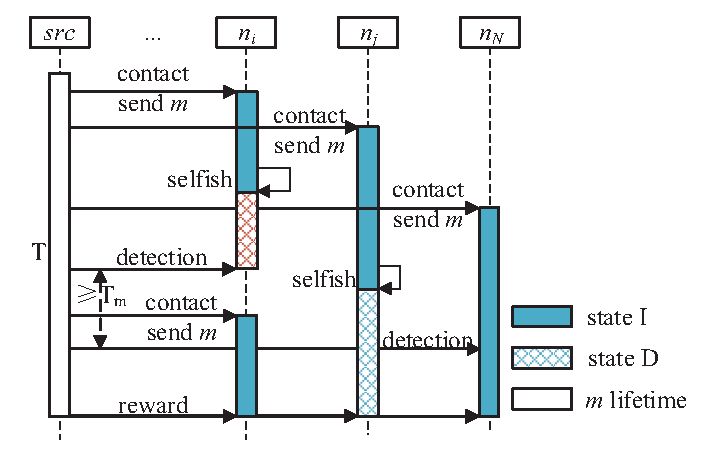
\includegraphics[width=0.47\textwidth]{fig/schedule.eps}}
     \caption{Sate transition by behaviors in the time sequence.}
     \label{fig:schedule}
\end{figure}
%1.Poisson process of contacts
%2.Poisson process of being selfish
$E(R(t))$ denotes the expected number of the relay nodes,
which have not contacted $src$ before time $t$.
$E(I(t))$ denotes the expected number of infected relay nodes,
which still carry the message at time $t$.
$E(D(t))$ denotes the expected number of selfish relay nodes,
which have discarded the message but are not known by $src$
at time $t$.
Similar to \cite{DBLP:journals/tcss/WuDH18} and \cite{CC2007PerfAnaly},
the contacts between each pair of nodes including $src$
are assumed to occur according to the Poisson process,
in which the contact rate is $\lambda$.
The total number of relay nodes is $N$,
and $N=R(t)+I(t)+D(t)$, $\forall t \in [0, T]$.
We also assume the change rate of
becoming the selfish node is a constant value $\rho$.
The detection rate is $U(t)$,
$0 \le U(t) \le U_{m}$, $\forall t \in [0, T]$.
which is the control function.
For example, if the minimal circle
of once detection $T_{m}$ is that $2$ seconds,
the maximal detection rate is
that $U_{m} = \frac{1}{T_{m}} = 0.5$ times per second.
To simplify the denotations,
we use $R(t)$, $I(t)$ and $D(t)$ to
replace $E(R(t))$, $E(I(t))$ and $E(D(t))$,
respectively.
The whole process,
including contacts, detections and reward,
is shown in Fig.~\ref{fig:schedule}.
The contacts can make the nodes in state $R$ and state $D$
to become the state $I$.
The selfish behavior let the node discard the message
and still earn the messages until be detected.
After the message lifetime,
the reward can be calculated according to
the contacts and the detections recorded in $src$.
Then the main objective of our work is to
to solve the following problem,
\begin{equation}
\begin{small}
\label{eq:obj}
\begin{aligned}
Min: J &= \int_{0}^{T} (1-\alpha) D(t) + \alpha U(t) dt,
\end{aligned}
\end{small}
\end{equation}
which minimizes the linear combination of
the wasted reward and the detection cost through the weight $\alpha$, $0 \le \alpha \le 1$.
We can also get the total paid reward is
\begin{equation}
\begin{small}
\label{eq:reward}
\begin{aligned}
P &= \int_{0}^{T} \beta ( I(t) + D(t) )dt,
\end{aligned}
\end{small}
\end{equation}
where $\beta$ is the reward paid for the one node's message carrying in a unit of time.
